\documentclass{article}
\usepackage{tikz, comment}
\usepackage{pifont}
\usepackage{fontspec}
\usetikzlibrary{arrows, decorations.markings, decorations.pathreplacing}
\begin{comment}
:Title: Not defined yet
:Tags: pi;;area using polar coordinates, polar integral formula ;moment;cosine, cos ;polar form of a complex number
:Prob: 0.4136;0.4077;0.4011;0.396;0.3847
:Slug: No name yet

Description Here.........
\end{comment}
\begin{document}\centering

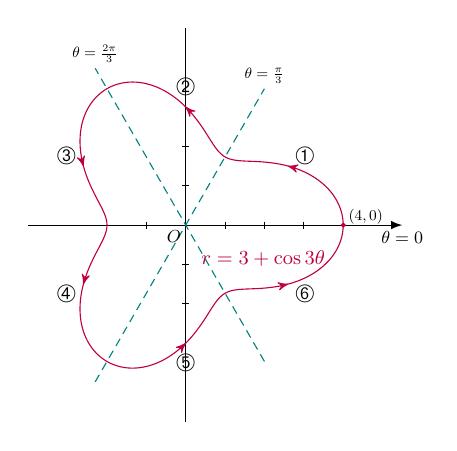
\begin{tikzpicture}[>=latex,xscale=.5*1, yscale=.5*1][font=\sf\small]

%\draw[xstep=1cm,ystep=1cm,color=gray!80] (0, -1) grid (8, 8);

\draw[->] (-4, 0) -- (5.5, 0)node[below, scale=0.7] {$\theta=0$};
\draw[] (0, -5) -- (0,5);

\draw[->, >=stealth', purple, samples=100, smooth, domain=0:1*pi/6, variable=\t]
plot ({(3+cos(3*\t r))*cos(\t r)}, {(3+cos(3*\t r))*sin(\t r)}) -- ({(3+cos(3*(1*pi/6) r))*cos((1*pi/6) r)}, {(3+cos(3*(1*pi/6) r))*sin((1*pi/6) r)});

\foreach \n in {1, 3, 5, 7, 9}
\draw[->, >=stealth', purple, samples=100, smooth, domain=(\n)*pi/6:(\n+2)*pi/6, variable=\t]
plot ({(3+cos(3*\t r))*cos(\t r)}, {(3+cos(3*\t r))*sin(\t r)}) -- ({(3+cos(3*((\n+2)*pi/6) r))*cos(((\n+2)*pi/6) r)}, {(3+cos(3*((\n+2)*pi/6) r))*sin(((\n+2)*pi/6) r)});

\draw[purple, samples=100, smooth, domain=11*pi/6:2*pi, variable=\t]
plot ({(3+cos(3*\t r))*cos(\t r)}, {(3+cos(3*\t r))*sin(\t r)});

\draw[purple, fill, xscale=1/1, yscale=1/1] ({4*1}, {0*1}) circle(0.05) node[black, right, xshift=0, yshift=3, scale=0.6] {$(4, 0)$};

\node[purple, xshift=28, yshift=-12, scale=0.8] at (0,0) {$r=3+\cos 3\theta$};

\foreach \x in {-1,1,2,3}
\draw (\x,2pt*1.25) -- (\x,-2pt*1.25)
node[anchor=north] {}%{\tiny$\x$}
;
\foreach \x in {}
\draw (\x,2pt*1.25) -- (\x,-2pt*1.25)
node[anchor=south] {\tiny$\x$}
;
\foreach \y in {-2,-1,1,2}
\draw (-2pt*1.25,\y) -- (2pt*1.25,\y)
node[anchor=east] {}%{\tiny $\y$}
;

\node at ({3.5*cos((1*pi/6) r)}, {3.5*sin((1*pi/6) r)}) {\ding{192}};
\node at ({3.5*cos((3*pi/6) r)}, {3.5*sin((3*pi/6) r)}) {\ding{193}};
\node at ({3.5*cos((5*pi/6) r)}, {3.5*sin((5*pi/6) r)}) {\ding{194}};
\node at ({3.5*cos((7*pi/6) r)}, {3.5*sin((7*pi/6) r)}) {\ding{195}};
\node at ({3.5*cos((9*pi/6) r)}, {3.5*sin((9*pi/6) r)}) {\ding{196}};
\node at ({3.5*cos((11*pi/6) r)}, {3.5*sin((11*pi/6) r)}) {\ding{197}};

\draw[densely dashed, teal, samples=100, smooth, domain=-2.3:2, variable=\x]
plot ({\x}, {tan(pi/3 r)*(\x)})node[above, black, scale=0.6] {$\theta=\frac{\pi}{3}$};

\draw[densely dashed, teal, samples=100, smooth, domain=2:-2.3, variable=\x]
plot ({\x}, {tan(2*pi/3 r)*(\x)})node[above, black, scale=0.6] {$\theta=\frac{2\pi}{3}$};

\node[scale=0.7] at (-0.3/1, -0.3/1) {$O$};

\end{tikzpicture}
\end{document}